\documentclass[border=5pt]{standalone}
\usepackage{fontspec,xeCJK,amsmath,amssymb,tikz,graphicx}
\usetikzlibrary{arrows.meta,calc}
\setmainfont{Arial}\setCJKmainfont{PingFang SC}
\definecolor{ink}{HTML}{203340}
\definecolor{blue}{HTML}{1680AC}
\definecolor{pale}{HTML}{EEF7FA}
\definecolor{warm}{HTML}{BF692A}
\definecolor{cream}{HTML}{FFF4E8}
\definecolor{line}{HTML}{D6E2E7}
\begin{document}
\begin{tikzpicture}[x=1cm,y=1cm,every node/.style={font=\fontsize{10}{13}\selectfont,text=ink},
box/.style={draw=line,rounded corners=5pt,fill=white,line width=.6pt},
flow/.style={-{Stealth[length=5pt]},line width=1pt,draw=blue},
update/.style={-{Stealth[length=5pt]},line width=1pt,dashed,draw=warm}]
\path[use as bounding box] (0,0) rectangle (10.5,34.7);
\fill[pale] (0,0) rectangle (10.5,34.7);
\node[font=\fontsize{20}{24}\selectfont\bfseries] at (5.25,34) {CLIP：图与文字怎么对上号？};
\node[font=\fontsize{10}{12}\selectfont,text=blue] at (5.25,33.4) {训练找配对 · 推理换类别文字};

\draw[box] (.55,28.2) rectangle (9.95,32.9);
\node[anchor=west,font=\fontsize{12}{14}\selectfont\bfseries] at (.85,32.5) {A　数据｜一批 $N$ 对图文};
\node at (2,30.8) {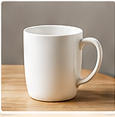
\includegraphics[width=1.9cm,height=1.8cm]{cup.png}};
\node at (5.25,30.8) {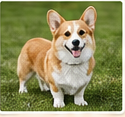
\includegraphics[width=1.9cm,height=1.8cm]{dog.png}};
\node at (8.45,30.8) {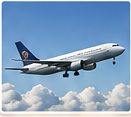
\includegraphics[width=1.9cm,height=1.8cm]{plane.png}};
\node[align=center,font=\fontsize{9}{11}\selectfont] at (2,29.35) {图 $x_1$：杯子\\配文 $y_1$：a cup};
\node[align=center,font=\fontsize{9}{11}\selectfont] at (5.25,29.35) {图 $x_2$：狗\\配文 $y_2$：a dog};
\node[align=center,font=\fontsize{9}{11}\selectfont] at (8.45,29.35) {图 $x_3$：飞机\\配文 $y_3$：a plane};
\node[font=\fontsize{9}{11}\selectfont,text=warm] at (5.25,28.6) {示意 $N=3$；预训练数据为 4 亿对互联网图文};
\draw[flow] (3,28.2)--(3,27.5);
\draw[flow] (7.5,28.2)--(7.5,27.5);

\draw[box] (.55,19.3) rectangle (9.95,27.5);
\node[anchor=west,font=\fontsize{12}{14}\selectfont\bfseries] at (.85,27.05) {B　双编码器｜用 ViT-B/32 看尺寸};
\draw[fill=pale,draw=line,rounded corners] (.85,20.7) rectangle (5.05,26.5);
\draw[fill=cream,draw=line,rounded corners] (5.45,20.7) rectangle (9.65,26.5);
\node[align=center,text=blue] at (2.95,26.05) {图像 $x_i$\\$224\times224\times3$};
\node[align=center,text=warm] at (7.55,26.05) {配文 $y_i$\\BPE 分词、补齐};
\node[align=center,font=\fontsize{9.5}{12}\selectfont] at (2.95,25) {$32\times32$ 切块、线性嵌入\\49 块 + CLS：$50\times768$};
\node[align=center,font=\fontsize{9.5}{12}\selectfont] at (7.55,25) {token 嵌入 + 位置编码\\序列形状：$77\times512$};
\draw[flow] (2.95,24.65)--(2.95,24.25);
\draw[flow] (7.55,24.65)--(7.55,24.25);
\node at (2.95,24.1) {
\includegraphics[width=2cm]{image-encoder.png}};
\node at (7.55,24.1) {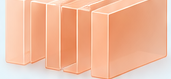
\includegraphics[width=2cm]{text-encoder.png}};
\node[align=center,font=\fontsize{9.5}{11}\selectfont] at (2.95,23.2) {12 层视觉 Transformer\\12 头注意力，取 CLS};
\node[align=center,font=\fontsize{9.5}{11}\selectfont] at (7.55,23.2) {12 层文本 Transformer\\8 头因果注意力，取 EOS};
\node[align=center,font=\fontsize{9.5}{11}\selectfont] at (2.95,22.22) {特征 768 维\\$W_I:768\times512$ 线性投影};
\node[align=center,font=\fontsize{9.5}{11}\selectfont] at (7.55,22.22) {特征 512 维\\$W_T:512\times512$ 线性投影};
\draw[flow] (2.95,21.95)--(2.95,21.6);
\draw[flow] (7.55,21.95)--(7.55,21.6);
\node[align=center] at (2.95,21.2) {L2 归一化 $\to u_i\in\mathbb R^{512}$};
\node[align=center] at (7.55,21.2) {L2 归一化 $\to v_i\in\mathbb R^{512}$};
\node[align=center,font=\fontsize{10}{13}\selectfont] at (5.25,20) {堆叠为 $U,V\in\mathbb R^{N\times512}$\\两路独立编码，最后比较方向};
\draw[flow] (5.25,19.3)--(5.25,18.6);

\draw[box] (.55,11.8) rectangle (9.95,18.6);
\node[anchor=west,font=\fontsize{12}{14}\selectfont\bfseries] at (.85,18.15) {C　配对损失｜行、列各做一次选择题};
\node at (5.25,17.5) {$S=\alpha UV^\top\in\mathbb R^{N\times N},\quad\alpha=e^t=1/\tau$};
\node[font=\fontsize{9}{11}\selectfont] at (5.25,16.9) {行是图像，列是文字；蓝色对角格是配对答案};
\foreach \rowindex in {0,1,2}{\foreach \colindex in {0,1,2}{
\pgfmathsetmacro{\xx}{3.95+\colindex*.85}\pgfmathsetmacro{\yy}{16.15-\rowindex*.85}
\pgfmathtruncatemacro{\ri}{\rowindex+1}\pgfmathtruncatemacro{\ci}{\colindex+1}
\ifnum\rowindex=\colindex\fill[blue!28] (\xx,\yy) rectangle ++(.8,-.8);\else\fill[pale] (\xx,\yy) rectangle ++(.8,-.8);\fi
\node[font=\fontsize{9}{11}\selectfont] at (\xx+.4,\yy-.4) {$S_{\ri,\ci}$};}}
\node[font=\fontsize{9}{11}\selectfont,text=blue] at (8.3,14.9) {横着挑文字};
\node[font=\fontsize{9}{11}\selectfont,text=blue] at (5.2,13.3) {竖着挑图像};
\draw[flow] (6.6,15.75)--(7.1,15.75);
\draw[flow] (4.35,13.75)--(4.35,13.4);
\node at (5.25,12.7) {$\mathcal L=\tfrac12(\mathrm{CE}(S,I_N)+\mathrm{CE}(S^\top,I_N))$};
\node[font=\fontsize{9}{11}\selectfont] at (5.25,12.2) {$I_N$ 表示对角配对目标；CE 为各行交叉熵的平均};
\draw[update] (.55,14)--(.22,14)--(.22,24)--(.85,24);
\draw[update] (9.95,14)--(10.25,14)--(10.25,24)--(9.65,24);
\node[rotate=90,text=warm,font=\fontsize{9}{11}\selectfont,fill=pale] at (.22,19) {梯度更新双编码器、投影与 $t$};

\draw[box] (.55,4.1) rectangle (9.95,11.1);
\node[anchor=west,font=\fontsize{12}{14}\selectfont\bfseries] at (.85,10.65) {D　零样本推理｜参数固定，文字换任务};
\node[align=center] at (5.25,9.8) {$K$ 个类别：杯子、狗、飞机\ldots\\填入 ``A photo of a \{label\}.''};
\draw[flow] (5.25,9.3)--(5.25,8.9);
\node[draw=line,fill=cream,rounded corners,align=center,minimum width=8.3cm] at (5.25,8.45) {同一文本编码器 + 投影 + L2 归一化\\类别权重 $W_{\rm cls}\in\mathbb R^{K\times512}$，提前缓存};
\draw[flow] (5.25,7.95)--(5.25,7.45);
\node[draw=line,fill=pale,rounded corners,align=center,minimum width=8.3cm] at (5.25,7) {新图 $x\to$ 同一图像编码器 $\to u\in\mathbb R^{512}$\\相似度 $s=\alpha uW_{\rm cls}^{\top}\in\mathbb R^K$};
\draw[flow] (5.25,6.5)--(5.25,6.05);
\node[align=center] at (5.25,5.65) {$p=\mathrm{softmax}(s)$，选最高分的类别\\换候选文字，就换分类器权重};
\node[font=\fontsize{9}{11}\selectfont,text=warm] at (5.25,4.75) {多提示模板：单位文本向量平均，再归一化};
\node[font=\fontsize{9}{11}\selectfont] at (5.25,4.35) {不走 C 的损失回路，不更新参数};
\draw[flow] (5.25,4.1)--(5.25,3.4);

\draw[box] (.55,.5) rectangle (9.95,3.4);
\node[anchor=west,font=\fontsize{12}{14}\selectfont\bfseries] at (.85,2.95) {E　实验与局限｜接口在哪儿管用？};
\node[align=center] at (5.25,2) {零样本：换类别 · 表征：固定特征换分类头\\分布偏移：换画风、视角、背景};
\node[align=center,font=\fontsize{9.5}{12}\selectfont,text=warm] at (5.25,1) {语义能接到机器人；空间定位和动作要另接结构\\§3\,实验 / §4\,重叠 / §5\,偏差 / §6\,边界};
\end{tikzpicture}
\end{document}
